% Options for packages loaded elsewhere
\PassOptionsToPackage{unicode}{hyperref}
\PassOptionsToPackage{hyphens}{url}
%
\documentclass[
  man]{apa6}
\usepackage{amsmath,amssymb}
\usepackage{iftex}
\ifPDFTeX
  \usepackage[T1]{fontenc}
  \usepackage[utf8]{inputenc}
  \usepackage{textcomp} % provide euro and other symbols
\else % if luatex or xetex
  \usepackage{unicode-math} % this also loads fontspec
  \defaultfontfeatures{Scale=MatchLowercase}
  \defaultfontfeatures[\rmfamily]{Ligatures=TeX,Scale=1}
\fi
\usepackage{lmodern}
\ifPDFTeX\else
  % xetex/luatex font selection
\fi
% Use upquote if available, for straight quotes in verbatim environments
\IfFileExists{upquote.sty}{\usepackage{upquote}}{}
\IfFileExists{microtype.sty}{% use microtype if available
  \usepackage[]{microtype}
  \UseMicrotypeSet[protrusion]{basicmath} % disable protrusion for tt fonts
}{}
\makeatletter
\@ifundefined{KOMAClassName}{% if non-KOMA class
  \IfFileExists{parskip.sty}{%
    \usepackage{parskip}
  }{% else
    \setlength{\parindent}{0pt}
    \setlength{\parskip}{6pt plus 2pt minus 1pt}}
}{% if KOMA class
  \KOMAoptions{parskip=half}}
\makeatother
\usepackage{xcolor}
\usepackage{graphicx}
\makeatletter
\def\maxwidth{\ifdim\Gin@nat@width>\linewidth\linewidth\else\Gin@nat@width\fi}
\def\maxheight{\ifdim\Gin@nat@height>\textheight\textheight\else\Gin@nat@height\fi}
\makeatother
% Scale images if necessary, so that they will not overflow the page
% margins by default, and it is still possible to overwrite the defaults
% using explicit options in \includegraphics[width, height, ...]{}
\setkeys{Gin}{width=\maxwidth,height=\maxheight,keepaspectratio}
% Set default figure placement to htbp
\makeatletter
\def\fps@figure{htbp}
\makeatother
\setlength{\emergencystretch}{3em} % prevent overfull lines
\providecommand{\tightlist}{%
  \setlength{\itemsep}{0pt}\setlength{\parskip}{0pt}}
\setcounter{secnumdepth}{-\maxdimen} % remove section numbering
% Make \paragraph and \subparagraph free-standing
\makeatletter
\ifx\paragraph\undefined\else
  \let\oldparagraph\paragraph
  \renewcommand{\paragraph}{
    \@ifstar
      \xxxParagraphStar
      \xxxParagraphNoStar
  }
  \newcommand{\xxxParagraphStar}[1]{\oldparagraph*{#1}\mbox{}}
  \newcommand{\xxxParagraphNoStar}[1]{\oldparagraph{#1}\mbox{}}
\fi
\ifx\subparagraph\undefined\else
  \let\oldsubparagraph\subparagraph
  \renewcommand{\subparagraph}{
    \@ifstar
      \xxxSubParagraphStar
      \xxxSubParagraphNoStar
  }
  \newcommand{\xxxSubParagraphStar}[1]{\oldsubparagraph*{#1}\mbox{}}
  \newcommand{\xxxSubParagraphNoStar}[1]{\oldsubparagraph{#1}\mbox{}}
\fi
\makeatother
% definitions for citeproc citations
\NewDocumentCommand\citeproctext{}{}
\NewDocumentCommand\citeproc{mm}{%
  \begingroup\def\citeproctext{#2}\cite{#1}\endgroup}
\makeatletter
 % allow citations to break across lines
 \let\@cite@ofmt\@firstofone
 % avoid brackets around text for \cite:
 \def\@biblabel#1{}
 \def\@cite#1#2{{#1\if@tempswa , #2\fi}}
\makeatother
\newlength{\cslhangindent}
\setlength{\cslhangindent}{1.5em}
\newlength{\csllabelwidth}
\setlength{\csllabelwidth}{3em}
\newenvironment{CSLReferences}[2] % #1 hanging-indent, #2 entry-spacing
 {\begin{list}{}{%
  \setlength{\itemindent}{0pt}
  \setlength{\leftmargin}{0pt}
  \setlength{\parsep}{0pt}
  % turn on hanging indent if param 1 is 1
  \ifodd #1
   \setlength{\leftmargin}{\cslhangindent}
   \setlength{\itemindent}{-1\cslhangindent}
  \fi
  % set entry spacing
  \setlength{\itemsep}{#2\baselineskip}}}
 {\end{list}}
\usepackage{calc}
\newcommand{\CSLBlock}[1]{\hfill\break\parbox[t]{\linewidth}{\strut\ignorespaces#1\strut}}
\newcommand{\CSLLeftMargin}[1]{\parbox[t]{\csllabelwidth}{\strut#1\strut}}
\newcommand{\CSLRightInline}[1]{\parbox[t]{\linewidth - \csllabelwidth}{\strut#1\strut}}
\newcommand{\CSLIndent}[1]{\hspace{\cslhangindent}#1}
\ifLuaTeX
\usepackage[bidi=basic]{babel}
\else
\usepackage[bidi=default]{babel}
\fi
\babelprovide[main,import]{english}
% get rid of language-specific shorthands (see #6817):
\let\LanguageShortHands\languageshorthands
\def\languageshorthands#1{}
% Manuscript styling
\usepackage{upgreek}
\captionsetup{font=singlespacing,justification=justified}

% Table formatting
\usepackage{longtable}
\usepackage{lscape}
% \usepackage[counterclockwise]{rotating}   % Landscape page setup for large tables
\usepackage{multirow}		% Table styling
\usepackage{tabularx}		% Control Column width
\usepackage[flushleft]{threeparttable}	% Allows for three part tables with a specified notes section
\usepackage{threeparttablex}            % Lets threeparttable work with longtable

% Create new environments so endfloat can handle them
% \newenvironment{ltable}
%   {\begin{landscape}\centering\begin{threeparttable}}
%   {\end{threeparttable}\end{landscape}}
\newenvironment{lltable}{\begin{landscape}\centering\begin{ThreePartTable}}{\end{ThreePartTable}\end{landscape}}

% Enables adjusting longtable caption width to table width
% Solution found at http://golatex.de/longtable-mit-caption-so-breit-wie-die-tabelle-t15767.html
\makeatletter
\newcommand\LastLTentrywidth{1em}
\newlength\longtablewidth
\setlength{\longtablewidth}{1in}
\newcommand{\getlongtablewidth}{\begingroup \ifcsname LT@\roman{LT@tables}\endcsname \global\longtablewidth=0pt \renewcommand{\LT@entry}[2]{\global\advance\longtablewidth by ##2\relax\gdef\LastLTentrywidth{##2}}\@nameuse{LT@\roman{LT@tables}} \fi \endgroup}

% \setlength{\parindent}{0.5in}
% \setlength{\parskip}{0pt plus 0pt minus 0pt}

% Overwrite redefinition of paragraph and subparagraph by the default LaTeX template
% See https://github.com/crsh/papaja/issues/292
\makeatletter
\renewcommand{\paragraph}{\@startsection{paragraph}{4}{\parindent}%
  {0\baselineskip \@plus 0.2ex \@minus 0.2ex}%
  {-1em}%
  {\normalfont\normalsize\bfseries\itshape\typesectitle}}

\renewcommand{\subparagraph}[1]{\@startsection{subparagraph}{5}{1em}%
  {0\baselineskip \@plus 0.2ex \@minus 0.2ex}%
  {-\z@\relax}%
  {\normalfont\normalsize\itshape\hspace{\parindent}{#1}\textit{\addperi}}{\relax}}
\makeatother

\makeatletter
\usepackage{etoolbox}
\patchcmd{\maketitle}
  {\section{\normalfont\normalsize\abstractname}}
  {\section*{\normalfont\normalsize\abstractname}}
  {}{\typeout{Failed to patch abstract.}}
\patchcmd{\maketitle}
  {\section{\protect\normalfont{\@title}}}
  {\section*{\protect\normalfont{\@title}}}
  {}{\typeout{Failed to patch title.}}
\makeatother

\usepackage{xpatch}
\makeatletter
\xapptocmd\appendix
  {\xapptocmd\section
    {\addcontentsline{toc}{section}{\appendixname\ifoneappendix\else~\theappendix\fi: #1}}
    {}{\InnerPatchFailed}%
  }
{}{\PatchFailed}
\makeatother
\keywords{keywords\newline\indent Word count: X}
\DeclareDelayedFloatFlavor{ThreePartTable}{table}
\DeclareDelayedFloatFlavor{lltable}{table}
\DeclareDelayedFloatFlavor*{longtable}{table}
\makeatletter
\renewcommand{\efloat@iwrite}[1]{\immediate\expandafter\protected@write\csname efloat@post#1\endcsname{}}
\makeatother
\usepackage{lineno}

\linenumbers
\usepackage{csquotes}
\usepackage{fancyhdr}
\pagestyle{empty}
\thispagestyle{empty}
\usepackage{float}
\ifLuaTeX
  \usepackage{selnolig}  % disable illegal ligatures
\fi
\usepackage{bookmark}
\IfFileExists{xurl.sty}{\usepackage{xurl}}{} % add URL line breaks if available
\urlstyle{same}
\hypersetup{
  pdftitle={Proportional reasoning across formats},
  pdfauthor={Abhi Patel},
  pdflang={en-EN},
  pdfkeywords={keywords},
  hidelinks,
  pdfcreator={LaTeX via pandoc}}

\title{Proportional reasoning across formats}
\author{Abhi Patel\textsuperscript{}}
\date{}


\shorttitle{SHORT TITLE}

\affiliation{\phantom{0}}

\begin{document}
\maketitle

\section{Introduction}\label{introduction}

Comparing proportions is sometimes very hard! But, even infants seem to be able to do it a little bit. The purpose of this science project was better understand how well people compare proportions when the proportions are presented in different formats. The purpose of this class assignment is to take the R code and plots we've been generating over the last several weeks and put it all together into one poster format. In order to make this a cohesive and insightful poster, we have put together these three connected research questions.

Research Questions:\vspace{-1em}

\begin{enumerate}
  \item Does average performance vary across format type?
  \item Does average performance vary across numerator congruency status?
  \item Does numerator congruency vary across format type? (i.e., is there an interaction)
\end{enumerate}

\section{Methods}\label{methods}

A total of \(99\) adults participated in the study.

First, participants were introduced to a story about a magic ball and that the outcome (i.e., blue or orange) depended on the proportions. They were then asked to compare the proportions of different images.

In other words, participants were shown two images of the same kind at the same time and asked to decide which had a higher proportion of the shape (or dots) colored in blue.

\begin{figure}[h]
  \includegraphics[width=0.8\textwidth, height=0.51\textheight]{data/Probtask_trial.png}
  \caption{This is a figure.}
\end{figure}

\subsection{Data Analysis}\label{data-analysis}

The data analysis was conducted using the following R packages: dplyr (Wickham, François, Henry, \& Müller, 2024) for data wrangling and summarization, and ggplot2 (Wickham, Chang, et al., 2024) for data visualization.

\section{Results}\label{results}

\begin{enumerate}
\def\labelenumi{\arabic{enumi}.}
\tightlist
\item
  Does average performance vary across format type, ignoring all other aspects of the stimuli?
\end{enumerate}

\begin{figure}
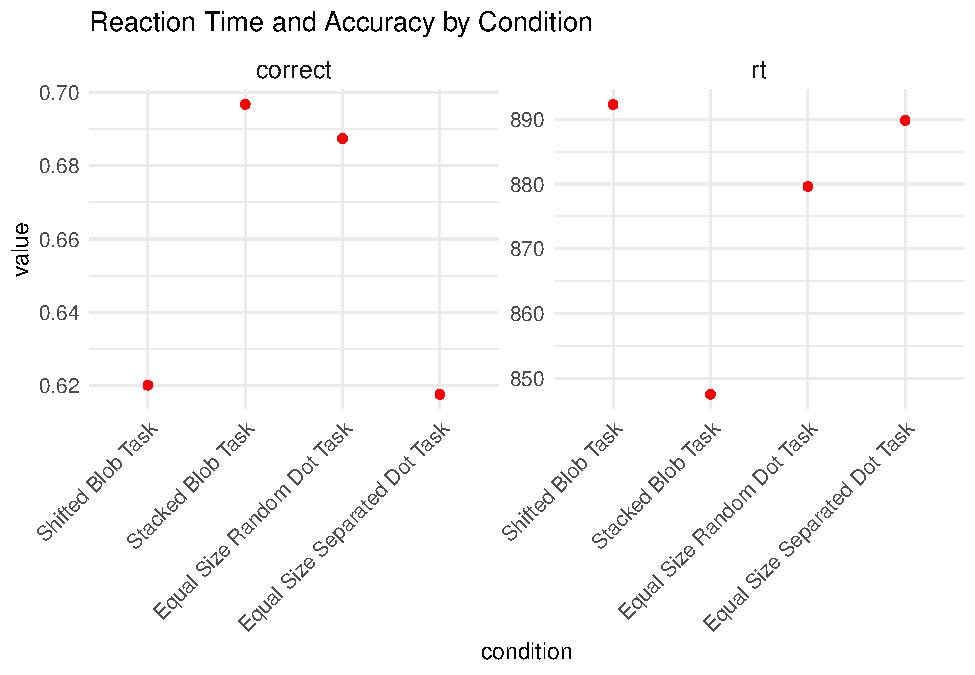
\includegraphics[width=0.6\linewidth,height=0.36\textheight]{Patel_WA11_files/figure-latex/assignment7-plot-1} \caption{Reaction Time and Accuracy by Condition}\label{fig:assignment7-plot}
\end{figure}

Average performance seems to vary. It seems that the tasks with the lower reaction times have higher accuracies.

\begin{enumerate}
\def\labelenumi{\arabic{enumi}.}
\setcounter{enumi}{1}
\tightlist
\item
  How are reaction time and accuracy related?
\end{enumerate}

\begin{figure}
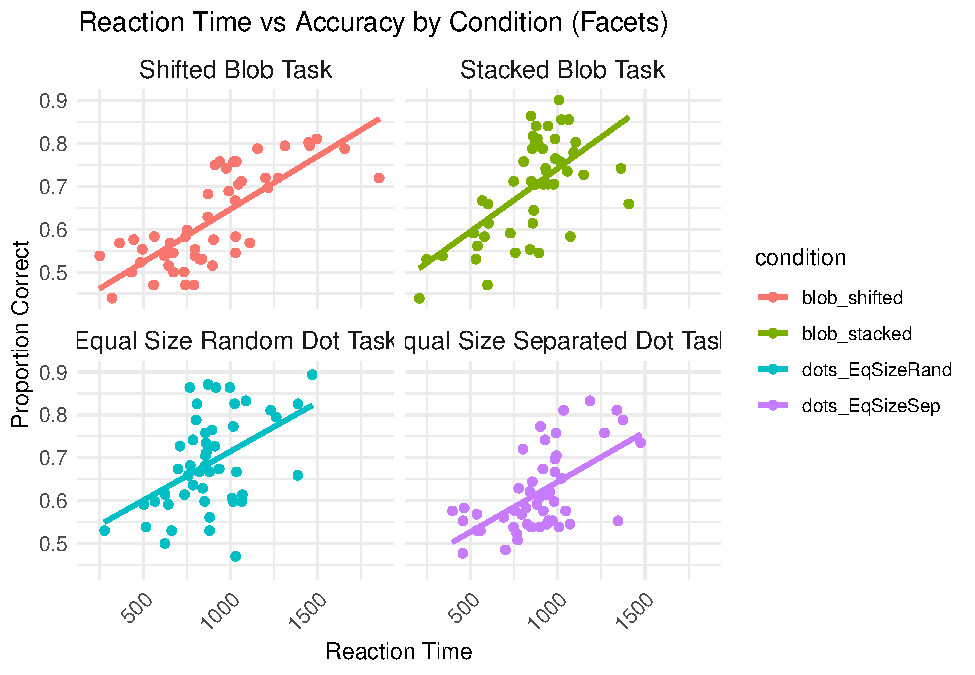
\includegraphics[width=0.6\linewidth,height=0.36\textheight]{Patel_WA11_files/figure-latex/assignment8-plot-1} \caption{Reaction Time vs. Accuracy by Condition}\label{fig:assignment8-plot}
\end{figure}

Reaction Time and Accuracy seem to be positively correlated with each other.

\begin{enumerate}
\def\labelenumi{\arabic{enumi}.}
\setcounter{enumi}{2}
\tightlist
\item
  How does numerator congruency interact with format type?
\end{enumerate}

\begin{figure}
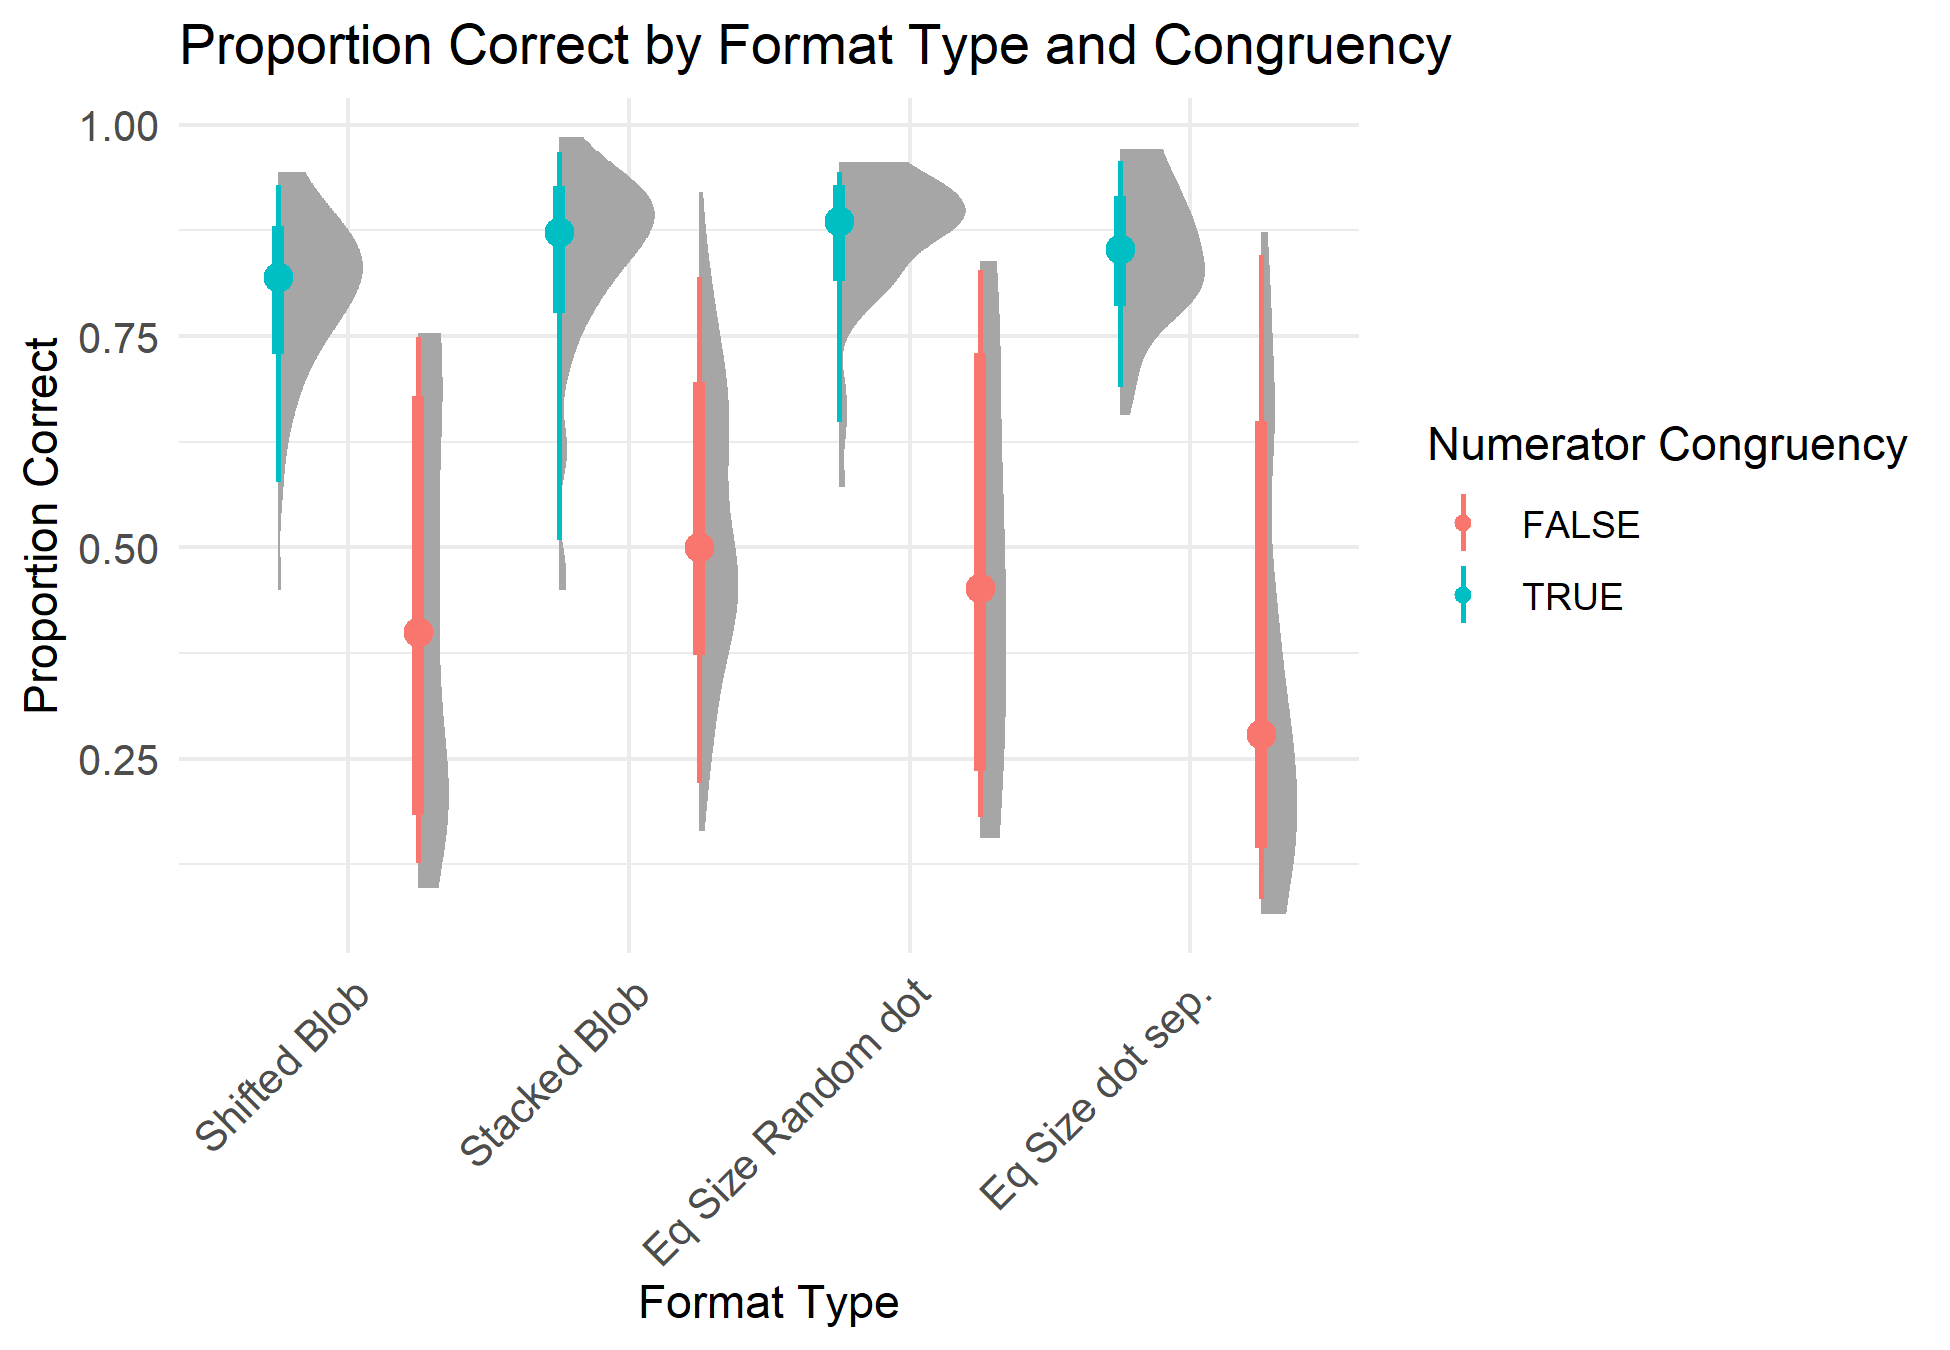
\includegraphics[width=0.6\linewidth,height=0.36\textheight]{Patel_WA11_files/figure-latex/assignment9-plot-1} \caption{Proportion Correct by Format Type and Congruency}\label{fig:assignment9-plot}
\end{figure}

Numerator Congruency interacts with format type by seeming to result in consistently higher accuracies in ``True'' rather than ``False''

\section{Discussion}\label{discussion}

Overall, we found that the tasks that resulted in the lower reaction times had the higher accuracies. This also makes sense as we found an overall positive relationship between reaction time and accuracy. To further investigate the accuracies, we looked at numerator congruency. We found that when the numerator congruency is true, there is overall higher accuracies than when it is false.
Provide two summaries of your experience during this assignment:

\begin{enumerate}
  \item \textbf{What was the most annoying or hardest thing about the assignment?} \\
  I found the most annoying thing to be altering graphs from previous assignments. It wasn't the worst, but it was just a bit tedious to do at once.
  
  \item \textbf{What was the most satisfying or fun thing about the assignment?} \\
  The poster looks cool. I like the way everything is organized in this format.
\end{enumerate}

\newpage

\section{References}\label{references}

\phantomsection\label{refs}
\begin{CSLReferences}{1}{0}
\bibitem[\citeproctext]{ref-R-ggplot2}
Wickham, H., Chang, W., Henry, L., Pedersen, T. L., Takahashi, K., Wilke, C., \ldots{} Dunnington, D. (2024). \emph{ggplot2: Create elegant data visualisations using the grammar of graphics}. Retrieved from \url{https://CRAN.R-project.org/package=ggplot2}

\bibitem[\citeproctext]{ref-R-dplyr}
Wickham, H., François, R., Henry, L., \& Müller, K. (2024). \emph{Dplyr: A grammar of data manipulation}. Retrieved from \url{https://CRAN.R-project.org/package=dplyr}

\end{CSLReferences}


\end{document}
